\documentclass{article}
\usepackage[utf8]{inputenc}
\usepackage[T1, T2A]{fontenc}
\usepackage[russian, english]{babel}
\usepackage{indentfirst}
\usepackage{graphicx}
\graphicspath{{./graphics/}}

\begin{document}
\begin{titlepage}
    \begin{center}
        \normalsize
        МГТУ им Н.Э. Баумана, кафедра ИУ5 \\
        \vspace*{1cm}
        \LARGE
        \textbf{Лабораторная работа №2 по дисцилине "РИП"}

        \vspace{0.5cm}
        Вариант 19
    \end{center}
    \vfill

    \begin{flushright}
        \textbf{Выполнил:} Никольский Даниил, ИУ5-51б \\
        \textbf{Проверил: } Гапанюк Юрий Евгеньевич, ИУ5 \\
    \end{flushright}
    \vspace{1.5cm}
    \begin{flushleft}
        \textbf{Дата: \today} \\
        \textbf{Подпись: Никольский Д.Р.} \\
    \end{flushleft}
\end{titlepage}

\tableofcontents
\newpage

\section{Задание}
\subsection{Задача 1}
Необходимо реализовать генераторы field и gen\_random. Генератор field последовательно выдает значения ключей словарей массива

\begin{enumerate}
    \item В качестве первого аргумента генератор принимает list, дальше через *args генератор принимает неограниченное кол-во аргументов.

    \item Если передан один аргумент, генератор последовательно выдает только значения полей, если поле равно None, то элемент пропускается

    \item Если передано несколько аргументов, то последовательно выдаются словари, если поле равно None, то оно пропускается, если все поля None, то пропускается целиком весь элемент

\end{enumerate}

Генератор gen\_random последовательно выдает заданное количество случайных чисел в заданном диапазоне

Пример: \\
gen\_random(1, 3, 5)должен выдать 5 чисел от 1 до 3, т.е. примерно 2, 2, 3, 2, 1

В ex\_1.py нужно вывести на экран то, что они выдают, с помощью кода в одну строку. Генераторы должны располагаться в librip/gen.py

\subsection{Задача 2}
Необходимо реализовать итератор, который принимает на вход массив или генератор и итерируется по элементам, пропуская дубликаты. Конструктор итератора также принимает на вход именной bool-параметр ignore\_case, в зависимости от значения которого будут считаться одинаковыми строки в разном регистре. По умолчанию этот параметр равен False. Итератор не должен модифицировать возвращаемые значения.

В ex\_2.py нужно вывести на экран то, что они выдают одной строкой. Важно продемонстрировать работу как с массивами, так и с генераторами (gen\_random).
Итератор должен располагаться в librip/iterators.py

\subsection{Задача 3}
Дан массив с положительными и отрицательными числами. Необходимо одной строкой вывести на экран массив, отсортированный по модулю. Сортировку осуществлять с помощью функции sorted

\subsection{Задача 4}
Необходимо реализовать декоратор print\_result, который выводит на экран результат выполнения функции. Файл ex\_4.py не нужно изменять.
Декоратор должен принимать на вход функцию, вызывать её, печатать в консоль имя функции, печатать результат и возвращать значение.
Если функция вернула список (list), то значения должны выводиться в столбик.
Если функция вернула словарь (dict), то ключи и значения должны выводить в столбик через знак равно

\subsection{Задача 5}
Необходимо написать контекстный менеджер, который считает время работы блока и выводит его на экран

\subsection{Задача 6}
Мы написали все инструменты для работы с данными. Применим их на реальном примере, который мог возникнуть в жизни. В репозитории находится файл data\_light.json. Он содержит облегченный список вакансий в России в формате json.
Структура данных представляет собой массив словарей с множеством полей: название работы, место, уровень зарплаты и т.д.
В ex\_6.py дано 4 функции. В конце каждая функция вызывается, принимая на вход результат работы предыдущей. За счет декоратора @print\_result печатается результат, а контекстный менеджер timer выводит время работы цепочки функций.
Задача реализовать все 4 функции по заданию, ничего не изменяя в файле-шаблоне. Функции f1-f3 должны быть реализованы в 1 строку, функция f4 может состоять максимум из 3 строк.

\begin{enumerate}
    \item Функция f1 должна вывести отсортированный список профессий без повторений (строки в разном регистре считать равными). Сортировка должна игнорировать регистр. Используйте наработки из предыдущих заданий.
    \item Функция f2 должна фильтровать входной массив и возвращать только те элементы, которые начинаются со слова “программист”. Иными словами нужно получить все специальности, связанные с программированием. Для фильтрации используйте функцию filter.
    \item Функция f3 должна модифицировать каждый элемент массива, добавив строку “с опытом Python” (все программисты должны быть знакомы с Python). Для модификации используйте функцию map.
    \item Функция f4 должна сгенерировать для каждой специальности зарплату от 100 000 до 200 000 рублей и присоединить её к названию специальности. Используйте zip для обработки пары специальность — зарплата.
\end{enumerate}
\newpage
\section{Исходные коды файлов}
\subsection{librip/gens.py}
\begin{verbatim}
import random


def field(val_list, *args):
    assert len(args) > 0
    for e in val_list:
        d = {}
        for a in args:
            if (a in e.keys()) and (len(args) == 1):
                yield e[a]
            elif a in e is not None:
                d[a] = e[a]
        if len(d) > 0 and len(args) > 1:
            yield d


def gen_random(beg, end, count):
    for i in range(count):
        yield random.randint(beg, end)

\end{verbatim}

\subsection{librip/iterators.py}
\begin{verbatim}
from typing import Union, Generator


class UniqueIterator:
    class GenericItem:
        def __init__(self, e):
            self.value = e
    
        def __hash__(self):
            return self.value.__hash__()

        def __eq__(self, other):
            return self.value == other.value
    
    class StringItem(GenericItem):
        def __init__(self, item: str, ignore_case: bool = False):
            super().__init__(item)
            self.ignore_case = ignore_case

        def __hash__(self) -> int:
            key = self.value if not self.ignore_case else self.value.lower()
            return key.__hash__()

        def __eq__(self, other) -> bool:
            return self.value == other.value if not self.ignore_case else self.value.lower() == other.value.lower()

    def __init__(self, obj: Union[list, Generator], ignore_case: bool = False, **kwargs):
        items = [
            UniqueIterator.StringItem(e, ignore_case)
            if isinstance(e, str)
            else
            UniqueIterator.GenericItem(e)
            for e in obj
        ]
        self._unique_items = iter([e.value for e in set(items)])

    def __iter__(self):
        return self

    def __next__(self):
        return next(self._unique_items)

\end{verbatim}

\subsection{librip/decorators.py}
\begin{verbatim}
import functools


def print_result(func):
    @functools.wraps(func)
    def wrapper(*args, **kwargs):
        print(func.__name__)
        result = func(*args, **kwargs)
        res_type = type(result)
        if res_type is list:
            for i in result:
                print(i)
        elif res_type is dict:
            for i in result.items():
                print(f'{i[0]}={i[1]}')
        else:
            print(result)
        return result

    return wrapper

\end{verbatim}

\subsection{librip/ctxmgr.py}
\begin{verbatim}
import time


class timer:
    def __init__(self):
        self.start = 0

    def __enter__(self):
        self.start = time.time()

    def __exit__(self, exc_type, exc_val, exc_tb):
        print(f'Run for {time.time() - self.start}')
\end{verbatim}

\subsection{ex\_1.py}
\begin{verbatim}
from lab2.librip.gens import field, gen_random

goods = [
    {'title': 'Ковер', 'price': 2000, 'color': 'green'},
    {'title': 'Диван для отдыха', 'price': 5300, 'color': 'black'},
    {'title': 'Стелаж', 'price': 7000, 'color': 'white'},
    {'title': 'Вешалка для одежды', 'price': 800, 'color': 'white'}
]

if __name__ == '__main__':
    print([e for e in field(goods, "title")])
    print([e for e in field(goods, "title", "price")])

    print([a for a in gen_random(1, 3, 5)])

\end{verbatim}
\subsection{ex\_2.py}
\begin{verbatim}
from lab2.librip.gens import gen_random
from lab2.librip.iterators import UniqueIterator
    
data1 = ['1', '1', '1', '1', 1, 2, 2, 2, 2, 2]
data2 = gen_random(1, 3, 10)
    
if __name__ == '__main__':
    i1 = UniqueIterator(data1)
    i2 = UniqueIterator(data2)
    
    print([e for e in i1])
    print([e for e in i2])
\end{verbatim}
\subsection{ex\_3.py}
\begin{verbatim}
if __name__ == '__main__':
data = [4, -30, 100, -100, 123, 1, 0, -1, -4]
print(sorted(data, key=lambda x: abs(x)))
\end{verbatim}

\subsection{ex\_4.py}
\begin{verbatim}
from lab2.librip.decorators import print_result


# Необходимо верно реализовать print_result
# и задание будет выполнено

@print_result
def test_1():
    return 1
    
    
@print_result
def test_2():
    return 'iu'
    
    
@print_result
def test_3():
    return {'a': 1, 'b': 2}
    
    
@print_result
def test_4():
    return [1, 2]
    
    
if __name__ == '__main__':
    test_1()
    test_2()
    test_3()
    test_4()        
\end{verbatim}

\subsection{ex\_5.py}
\begin{verbatim}
    from time import sleep
    from lab2.librip.ctxmgr import timer
    
    if __name__ == '__main__':
        with timer():
            sleep(5.5)    
\end{verbatim}
\subsection{ex\_6.py}
\begin{verbatim}
    import json
    import sys
    from lab2.librip.ctxmgr import timer
    from lab2.librip.decorators import print_result
    from lab2.librip.gens import field, gen_random
    from lab2.librip.iterators import UniqueIterator as unique
    
    path = sys.argv[1]
    
    # Здесь необходимо в переменную path получить
    # путь до файла, который был передан при запуске
    
    
    # Далее необходимо реализовать все функции по заданию, заменив `raise NotImplemented`
    # Важно!
    # Функции с 1 по 3 дожны быть реализованы в одну строку
    # В реализации функции 4 может быть до 3 строк
    # При этом строки должны быть не длиннее 80 символов
    
    @print_result
    def f1(arg):
        return list(unique(field(arg, "job-name"), ignore_case=True))
    
    
    @print_result
    def f2(arg):
        return list(filter(lambda s: "программист" in s, arg))
    
    
    @print_result
    def f3(arg):
        return list(map(lambda s: f"{s} с опытом Python", arg))
    
    
    @print_result
    def f4(arg):
        prof = gen_random(100000, 200000, len(arg))
        return list(map(lambda s: f'{s[0]}, зарплата {s[1]} руб.', zip(arg, prof)))
    
    
    if __name__ == '__main__':
        with open(path) as f:
            data = json.load(f)
    
        with timer():
            f4(f3(f2(f1(data))))
\end{verbatim}
\newpage
\section{Результаты выполнения}
Вывод функций f1, f2 и f3 в файле ex\_6.py опущен ввиду избыточности.

\begin{figure}[h!]
    \centering
    
\includegraphics[width=\textwidth]{ex1.png}
    \caption{ex\_1.py}
    \label{fig: ex1}
\end{figure}

\begin{figure}[h!]
    \centering
    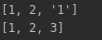
\includegraphics{ex2.png}
    \caption{ex\_2.py}
    \label{fig: ex2}
\end{figure}

\begin{figure}[h!]
    \centering
    
\includegraphics[width=\textwidth]{ex3.png}
    \caption{ex\_3.py}
    \label{fig: ex3}
\end{figure}

\begin{figure}[h!]
    \centering
    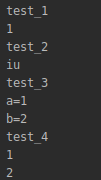
\includegraphics{ex4.png}
    \caption{ex\_4.py}
    \label{fig: ex4}
\end{figure}

\begin{figure}[h!]
    \centering
    
\includegraphics[width=\textwidth]{ex5.png}
    \caption{ex\_5.py}
    \label{fig: ex5}
\end{figure}
\begin{figure}[h!]
    \centering
    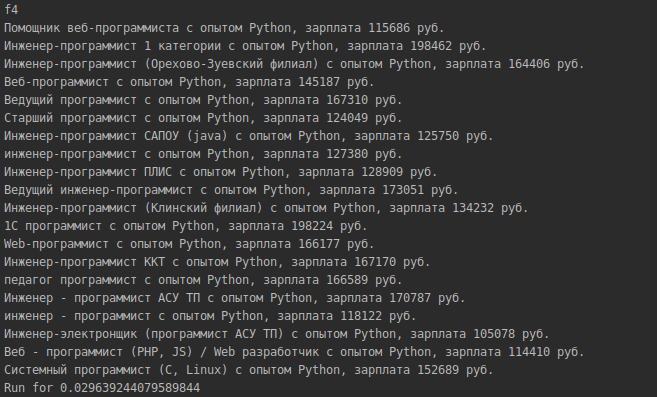
\includegraphics[width=\textwidth]{ex6.png}
    \caption{ex\_6.py}
    \label{fig: ex6}
\end{figure}
\end{document}